\section{Design}

Our design is split up in three modules. Every module is designed according to the MVC pattern.
\begin{description}
    \item[bohnanza] {Mostly an abstract module that contains logic for both the \gls{std} and
    \gls{hb} game.}
    \item[bohnanza-std] {A concrete module that uses the \emph{bohnanza} module in order to play
    the \gls{std} bohnanza game.}
    \item[bohnanza-hb] {A concrete module that uses the \emph{bohnanza} module in order to play the
    \gls{hb} bohnanza game.}
\end{description}

\subsection{Model}

\begin{figure}[h!]
    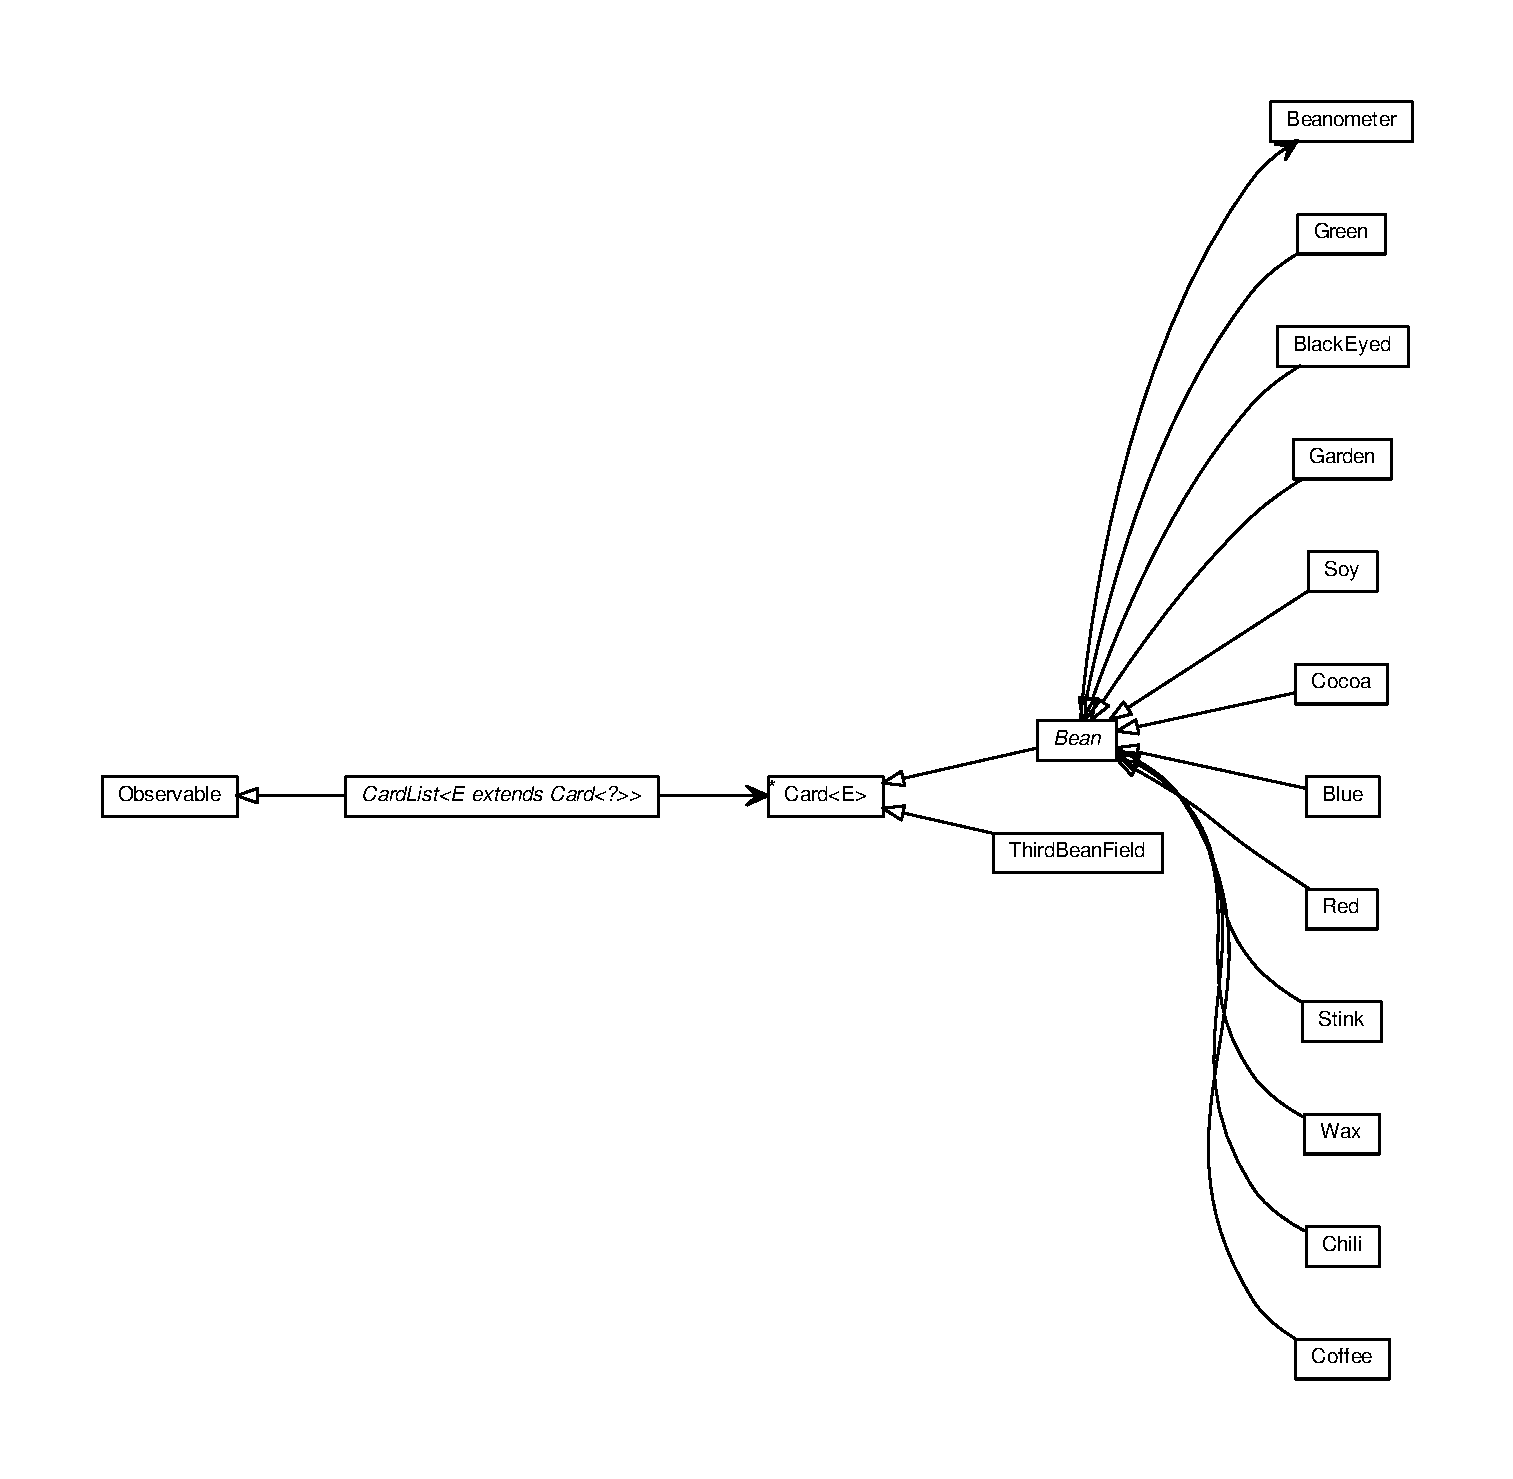
\includegraphics[width=\textwidth]{../umlgraph/CardGraph}
    \caption{Class diagram of the cards}
    \label{fig:design:cards}
\end{figure}

\begin{figure}[h!]
    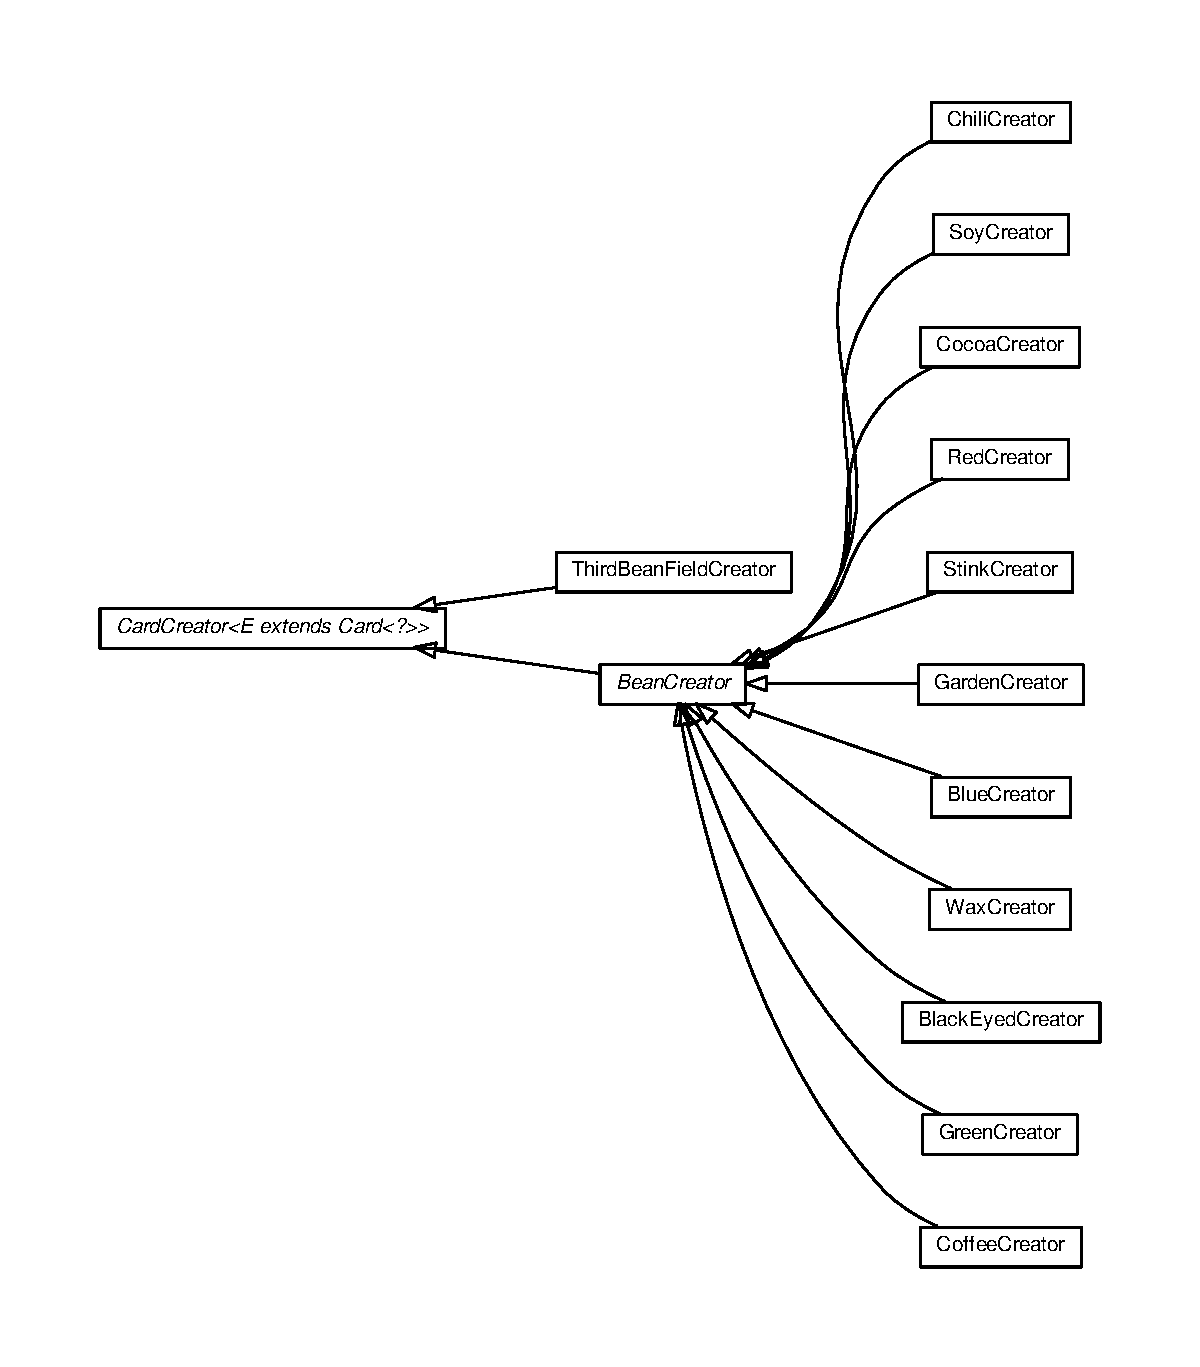
\includegraphics[width=\textwidth]{../umlgraph/CreatorGraph}
    \caption{Class diagram for the creation of cards}
    \label{fig:design:cards}
\end{figure}

\begin{figure}[h!] 
    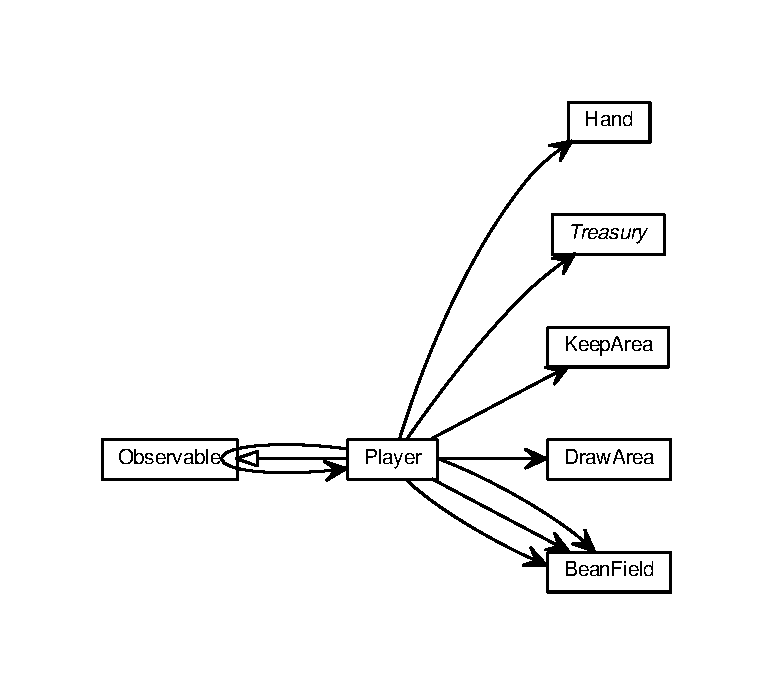
\includegraphics[width=\textwidth]{../umlgraph/PlayerGraph}
    \caption{Class diagram for the player and association to particular sets of cards}
    \label{fig:design:cards}
\end{figure}

\subsection{Controller}

\begin{figure}[h!]
    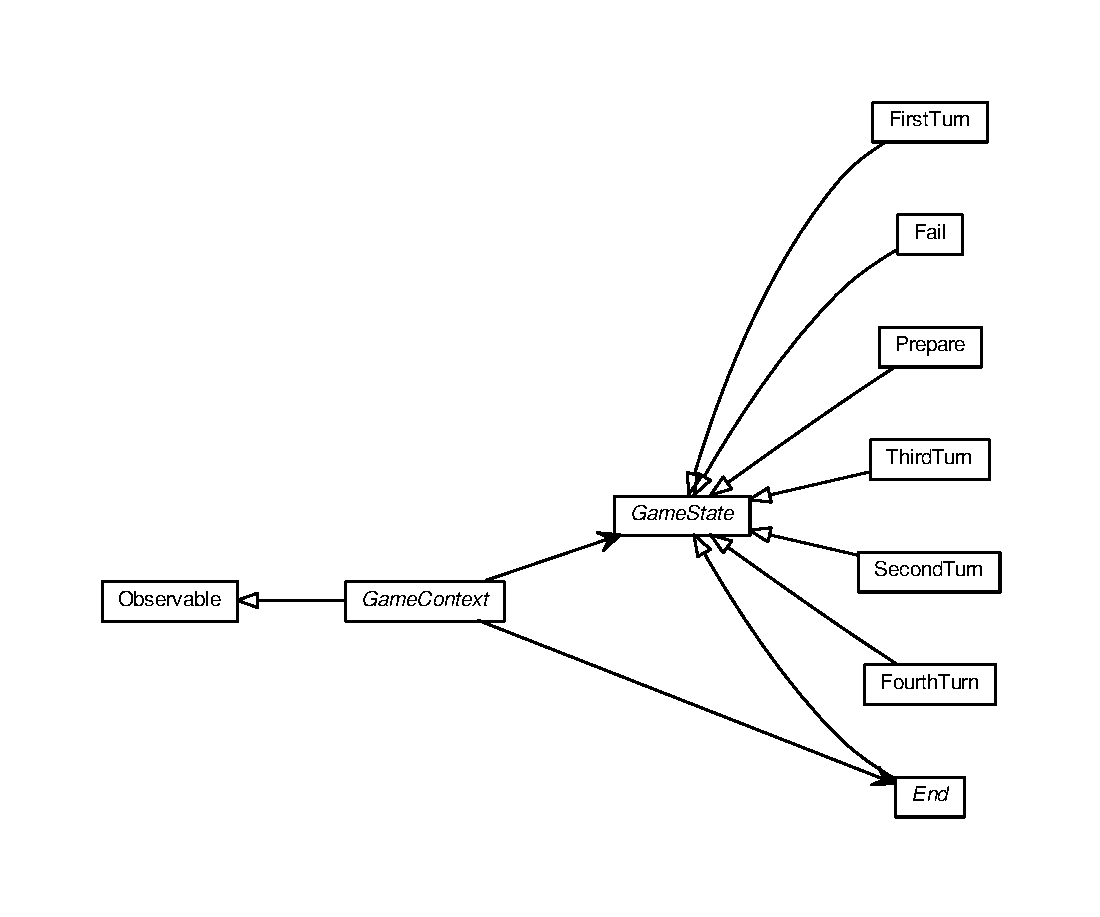
\includegraphics[width=\textwidth]{../umlgraph/StateGraph}
    \caption{Class diagram for controlling the state of the game}
    \label{fig:design:cards}
\end{figure}

\subsection{View}
Currently we support only a textual user interface. The \texttt{TUIView} class is an implementation
of a \texttt{View} interface. Creating a new interface like a graphical or a network would involve
implementing the \texttt{View} interface.

\subsection{Variations}
\subsubsection{User}
The user can specify during the startup of the application how many players there are using a
commandline option. For example \texttt{java bohnanza.BohnanzaStd -p=3} starts the BohnanzaStd
module with three players. Parsing commandline options is done using the Apache Commons CLI library.

\subsubsection{Developer}
Variability for the develop depends heavily on notion of dependency injection. Dependency injection
basically involves moving dependency resolution from a particular class to a framework dedicated to
dependeny injection. We use Guice\footnote{https://code.google.com/p/google-guice/} for this. If a
developer wants another variation of the application the developer can simply extend the
\texttt{BohnanzaModule} class and define other classes to inject. For example if a \texttt{Hand}
object needs to behave differently for a particular extension of Bohnanza one can extend
\texttt{Hand} and define the extension in extension of \texttt{BohnanzaModule}.

\begin{figure}[h!]
    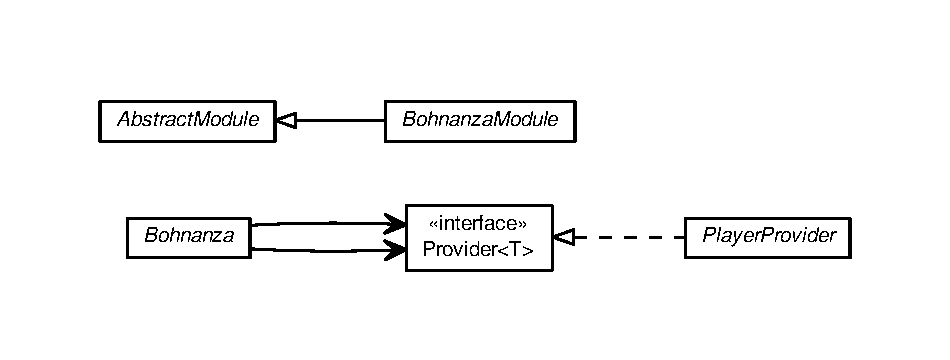
\includegraphics[width=\textwidth]{../umlgraph/ModuleGraph}
    \caption{Class diagram of classes involving dependency injection}
    \label{fig:design:cards}
\end{figure}
